%==============================================================================
% 8 RESULTS III: FIDELITY AGAINST EVERY BASELINE
% Plano: o modelo contra cinematica ideal, rSim (stock, e com atraso casado), MuJoCo
% rota a (embedding = gemeo) e rota b (sem sintonia, com atraso), grSim e ER-Force
% (teleporte cru, +atraso, pre-rolagem; tres sessoes: 10/09, 18/09, 20/09);
% repetibilidade entre sessoes (as tres sessoes lado a lado na tabela); condicao inicial (modelo com estados zerados 0.1137, pre-rolado 0.0406);
% atribuicao de Shapley; v0 causal; LOO; controle negativo bayesiano; heading.
% Baseline sintonizada (C3 ou rSim): so se a orientadora aprovar (WP3).
% Fontes: tab_journal_baselines, tab_journal_robustness, fig_journal_league_sims
% (geradas); CHANGELOG 2026-09-07 15:15 (C2a), 2026-09-10 02:11 (C2b),
% 2026-09-18 13:26 (C2b2 sessao 1, entrada do lote 1), 2026-09-20 11:43 (C2b2 sessao 2).
%==============================================================================
\section{Results III: fidelity against physics and league simulators}
\label{sec:res-fidelity}

% ==============================================================================
% tab_journal_baselines: generated by `dtssl analysis run journal_tables` (dtssl.analysis.journal_tables).
% Do not edit by hand: re-run the generator. Sources:
%   results/epos_eang_three_models_20260810_1022.md
%   results/negcontrol_perevent_20260810_1035.md
%   results/eval_rsim_delay_ablation_20260809_2154.md
%   results/backends_holdout_20260907_1515.md
%   results/backends_holdout_20260907_1515.csv
%   results/protocol_holdout_20260910_0211.json
%   results/protocol_holdout_20260918_1326.json
%   results/protocol_holdout_20260920_1143.json
% ==============================================================================
% Needs \usepackage{booktabs,adjustbox}.
\begin{table*}[t]
\centering
\caption{Every baseline scored on the same windows and metric as the identified model.}
\label{tab:baselines}
\small
\begin{adjustbox}{max width=\textwidth}
\begin{tabular}{llcccc}
\toprule
plant & session & $e_{\mathrm{pos}}$ per window (m) & $e_{\mathrm{pos}}$ per event (m) & model wins & $p$ \\
\midrule
Identified model & in process & 0.0388 & 0.0421 & -- & -- \\
Model, states zeroed at $t_0$ & in process & 0.1137 & -- & -- & -- \\
Model, pre-rolled & in process & 0.0406 & -- & -- & -- \\
\midrule
Ideal kinematics & in process & 0.1005 & 0.1177 & 10/10 & $9.8\times10^{-4}$ \\
rSim, stock parameters & in process & 0.1293 & -- & -- & -- \\
rSim, stock + matched delay & in process & 0.1822 & -- & -- & -- \\
MuJoCo, velocity-driven (route a) & in process & 0.0388 & 0.0421 & 7/10 & $0.22$ \\
MuJoCo rollers, untuned (route b) & in process & 0.0729 & 0.0791 & 10/10 & $9.8\times10^{-4}$ \\
MuJoCo rollers + delay & in process & 0.0477 & 0.0487 & 9/10 & $9.8\times10^{-3}$ \\
\midrule
grSim, teleport (rest) & 09-10 / 09-18 / 09-20 & 0.2389 / 0.2421 / 0.2329 & 0.2341 / 0.2398 / 0.2299 & 10/10 / 10/10 / 10/10 & $9.8\times10^{-4}$ \\
grSim + delay & 09-10 & 0.2335 & 0.2345 & 10/10 & $9.8\times10^{-4}$ \\
grSim, pre-rolled & 09-18 / 09-20 & 0.0996 / 0.0809 & 0.1106 / 0.0975 & 10/10 / 10/10 & $9.8\times10^{-4}$ \\
ER-Force, teleport & 09-10 / 09-18 / 09-20 & 0.0881 / 0.0856 / 0.0874 & 0.1006 / 0.1023 / 0.0995 & 10/10 / 10/10 / 10/10 & $9.8\times10^{-4}$ \\
ER-Force + delay & 09-10 & 0.0555 & 0.0555 & 9/10 & $2.0\times10^{-3}$ \\
ER-Force, pre-rolled & 09-18 / 09-20 & 0.0934 / 0.0940 & 0.1114 / 0.1114 & 10/10 / 10/10 & $9.8\times10^{-4}$ \\
\bottomrule
\end{tabular}
\end{adjustbox}

\vspace{2pt}
\parbox{\linewidth}{\footnotesize Median position error at $h_{\mathrm{ref}} = 0.4$ s on the translation-dominated hold-out windows: over windows, and the median of the ten per-event medians; model wins and one-sided paired Wilcoxon $p$ per event (model $<$ plant; $p$ shown once where equal in every session). Sessions are dates of the real-time protocol replays (2026). Dashes: not computed per event in the artefact.}
\end{table*}


\begin{figure*}[t]
  \centering
  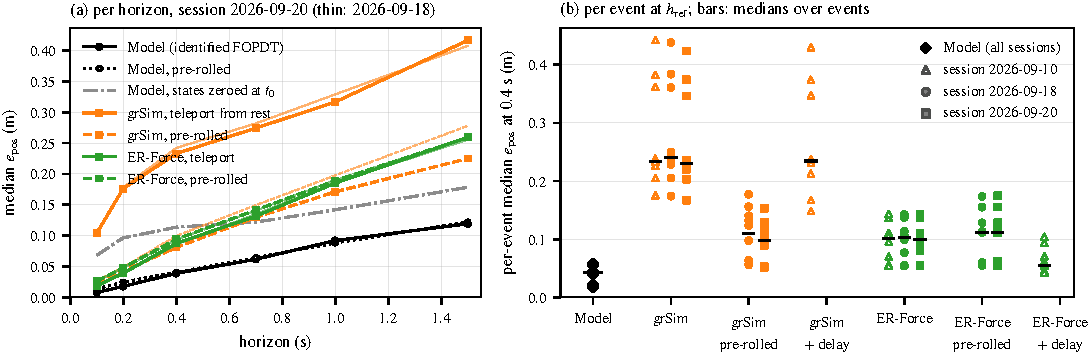
\includegraphics[width=\textwidth]{fig_journal_league_sims.pdf}
  \caption{League simulators replayed through the simulation protocol on the hold-out windows. (a) Median position error per horizon; the pre-roll lets each simulator reach the anchor with its own dynamics. (b) Per-event medians at the reference horizon in every session.}
  \label{fig:league}
\end{figure*}

% ==============================================================================
% tab_journal_robustness: generated by `dtssl analysis run journal_tables` (dtssl.analysis.journal_tables).
% Do not edit by hand: re-run the generator. Sources:
%   results/ablation_orderfree_20260810_1021.md
%   results/causal_ic_check_20260810_1102.md
%   results/gate_window_vs_event_20260810_1743.md
%   results/negcontrol_perevent_20260810_1035.md
%   results/eval_rsim_delay_ablation_20260809_2154.md
%   results/loo_translational_20260810_1743.md
% ==============================================================================
% Needs \usepackage{booktabs,adjustbox}.
\begin{table*}[t]
\centering
\caption{Robustness of the fidelity result.}
\label{tab:robustness}
\small
\begin{adjustbox}{max width=\textwidth}
\begin{tabular}{lp{0.62\linewidth}}
\toprule
check & result (position error at $h_{\mathrm{ref}} = 0.4$ s unless stated) \\
\midrule
Order-free attribution of the gain over ideal kinematics (0.0617 m) & $\tau$ 55\%, $T_d$ 43\%, $K$ 2\% \\
Measured initial velocity & constant-velocity extrapolation 0.1600 m; model from rest 0.1137 m; model with measured velocity 0.0388 m \\
Strictly causal initial velocity & 0.0468 m (central 0.0388 m); per-event gap +0.0706 m, 10/10, $p = 9.8\times10^{-4}$ \\
Unit of analysis & windows ($n=49$): gap +0.0541 m, $p = 1.2\times10^{-8}$, $r_{rb} = 0.633$; events ($n=10$): gap +0.0689 m, $p = 9.8\times10^{-4}$, $r_{rb} = 1.000$ \\
Negative control (9-parameter Bayesian calibration) & per-event gap +0.0038 m, 7/10, $p = 0.042$, $r_{rb} = 0.40$ \\
rSim with the model's transport delay & 0.1293 $\rightarrow$ 0.1822 m (gap widens) \\
Leave-one-event-out fit & $v_x$ $84.3\pm2.0$\% (4 folds); $v_y$ $82.8\pm2.7$\% (13 folds) \\
\bottomrule
\end{tabular}
\end{adjustbox}
\end{table*}


\pending{text of the section.}
